\documentclass[amssymb,twocolumn,aps]{revtex4}

% allows special characters (including æøå)
\usepackage[utf8]{inputenc}
%\usepackage [norsk]{babel} %if you write norwegian
\usepackage[english]{babel}  %if you write english

\usepackage{physics,amssymb}  % mathematical symbols (physics imports amsmath)
\usepackage{graphicx}         % include graphics such as plots
\usepackage[table]{xcolor}
\usepackage{xcolor}           % set colors
\usepackage{hyperref}         % automagic cross-referencing 
\usepackage{float}			  % force placement of tables and figures

\begin{document}
	
\title{Report Template \\
    \normalsize FYS-STK3155 - Project X}
\date{\today}               
\author{Student}
\affiliation{University of Oslo}

\newpage
	
\begin{abstract}
The abstract gives the reader a quick overview of what has been done and the most important results. Try to be to the point and state your main findings. It could be structured as follows:
\begin{itemize}
    \item Short introduction to topic and why its important
    \item Introduce a challenge or unresolved issue with the topic (that you will try to solve)
    \item What have you done to solve this
    \item Main Results
    \item The implications
\end{itemize}
\end{abstract}

\maketitle

\section{Introduction}
When you write the introduction you should focus on the following aspects:
\begin{itemize}
    \item Motivate the reader, the first part of the introduction gives always a motivation and tries to give the overarching ideas. Citing some central ideas or problems in the literature is a good idea here. \cite{compfys}\cite{eigenvalue}\cite{hein, hastie}
    \item What you have done, with a focus on choice of problem and method, and why these were chosen.
    \item The structure of the report, how it is organized. List the sections, and very briefly describe what is in them and how they fit together.
\end{itemize}
    
\section{Methods}\label{section:methods}

\subsection{Method 1/X}

\begin{itemize}
    \item Describe the methods and algorithms, including the motivation for using them and their applicability to the problem
    \item Derive central equations when appropriate, the text is the most important part, not the equations.
\end{itemize}

\subsection{Implementation}

\begin{itemize}
    \item Explain how you implemented the methods and also say something about the structure of your algorithm and present very central parts of your code, not more than 10 lines
    \item You should plug in some calculations to demonstrate your code, such as selected runs used to validate and verify your results. A reader needs to understand that your code reproduces selected benchmarks and reproduces previous results, either numerical and/or well-known closed form expressions.
\end{itemize}

\subsection{Use of AI tools}
	
\begin{itemize}
    \item Describe how AI tools like ChatGPT were used in the production of the code and report.
\end{itemize}
	
\section{Results and Discussion}\label{section:results} 

\begin{itemize}
    \item Present your results
    \item Give a critical discussion of your work and place it in the correct context.
    \item Relate your work to other calculations/studies
    \item An eventual reader should be able to reproduce your calculations if she/he wants to do so. All input variables should be properly explained.
    \item Make sure that figures\ref{fig:puppy} and tables contain enough information in their captions, axis labels etc. so that an eventual reader can gain a good impression of your work by studying figures and tables only.
\end{itemize}

\begin{figure}[h]
    \centering
    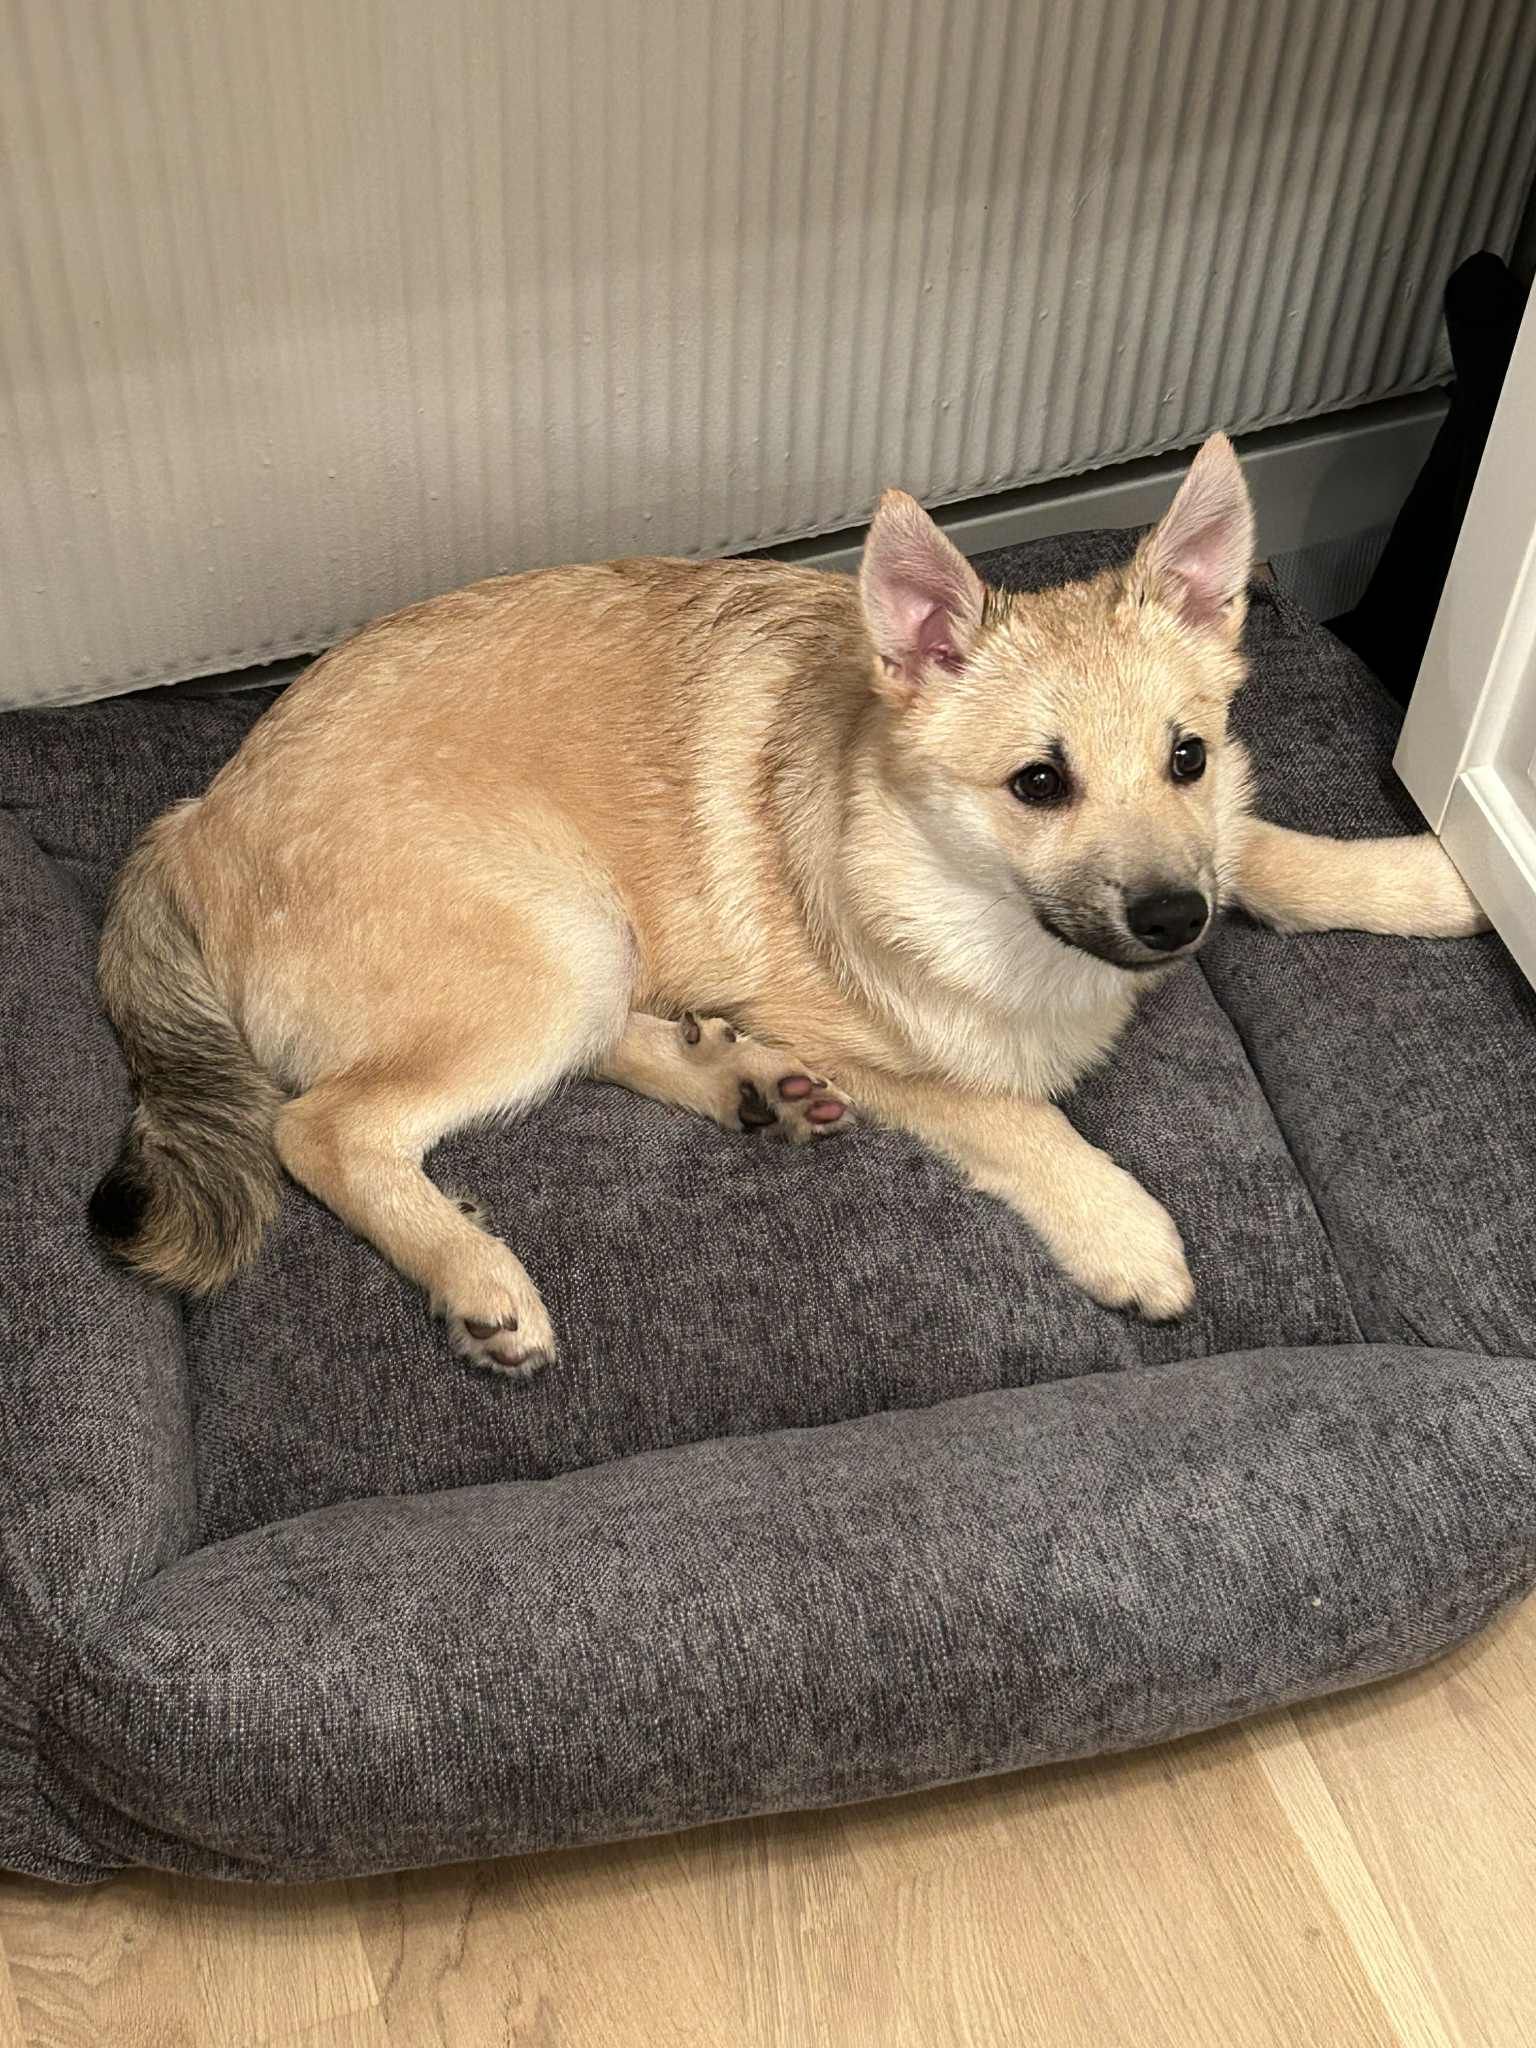
\includegraphics[width=0.5\linewidth]{Figures/puppy.jpg}
    \caption{My dog.}
    \label{fig:puppy}
\end{figure}


\section{Conclusion}\label{section:conclusion} 
\begin{itemize}
    \item State your main findings and interpretations
    \item Try to discuss the pros and cons of the methods and possible improvements
    \item State limitations of the study
    \item Try as far as possible to present perspectives for future work
\end{itemize}

\bibliography{biblio}

\end{document}
